\chapter{Introduction}
\label{ch:intro}

\section{Purpose }
The purpose of this document is to describe the Software Requirements Specifications (SRS) of the proposed application (Tutor-Hub). This will be the 1st release of this app. The application consists of two main parts, the web application and the backend server. Application architecture design, scopes, functions and its integration with existing systems at application designs are the core elements to be described in this document. This document provides a complete understanding of what is to be expected from the application. Clear understanding of the application and its functionalities will allow for the correct software to be developed for the end users. It can be used for future development of the application. This document provides the foundation for the design, construction, and testing of the application.

\section{Intended Audience}
The SRS described in this document is to be used by the group members and course instructor for developing the application. The group members will use the SRS to fully understand the expectations and requirements needed in the application. They will be able to use this SRS as a reference to see if the group members are constructing the application as per expectations.

This document is intended for developers (group members), instructor and TA of the course. The modification and maintenance of the app will be done by the team members. The team members and faculty will have access to this SRS.

\section{Intended Use}
This document will be used to develop a web-based tutor finder app where tutors and students will be able to find their intended tuition/tutor. The development team will use this SRS document as the basis for their entire project. Every person involved in development will follow the framework of this document to ensure requirements are fulfilled. Developers (group members) will use this document to understand the requirements of users and how they will use and interact with the system to be developed in order to perform their activities. The specification for software to be developed, which include functionalities, non-functional requirements, and software architecture can be found in this document. 
Group members along with the instructor will use this document to systematically plan the functional and security testing strategy of the application. Group members will also use the SRS to design the use case flow structure and content to show how the application can be used in the most effective way. It has to be delivered as end-user manual and technical documentations that covers all the requirement aspects proposed. Furthermore, the document will be used to minimize development time and cost.
\section{Product Scope}
Manual tuition quest is an old process in today's world of technology. The Tutor Hub web application will provide a new way of seeking suitable tutors for students as well as suitable jobs for the tutors. 
The main benefits of this web application will be:
      
\begin{enumerate}
\item The web application will be interactive and create job sectors for the tutors.   
\item The design will be simple so that minimal educated users can use them easily.
\item The tutors/ tuition's will be recommended by the nearby or selected location of the user. 
\item  A student will be able to see the main information like expected salary, preferable classes of the tutors. This will save time as they will be viewing the keywords only in the homepage and can compare this information with other tutors' information.
\item The tutor can form a batch for a specific subject and can upload online materials in that platform.
\end{enumerate}

\section{Risk Definition}
\begin{enumerate}
\item       There are chances that the requirements won't be fulfilled.
\item       We can face some problems in the unit testing.
\item       We also can face problems while implementing AI.
\end{enumerate}




\chapter{Overall Description}
\label{Overall Description}

\section{User Classes and Characteristics}
%%% User classes and Characteristics Table %%%

\textbf{"Tutor-Hub"} is an Online Tutor Finder System used by many people Locally. The main users of the Project system under development will be Tutors and students and Parents.
\begin{center}
\setlength{\tabcolsep}{1.0cm}
\renewcommand{\arraystretch}{1.5}
    \begin{table}[ht]
        \centering
        \begin{tabular}{|m{70pt}|p{9cm}|}
            \hline
                \textbf{No}  & \textbf{ User class and Characteristics} \\
            \hline
                	\textbf{1 }& 
                     	\textbf{Student} \newline
                       \textbf{  \underline{Description }:} \newline
                		The majority of students shall use this application to find private tutor. The technical
                        experience of these users should not matter as the system will be straightforward and
                        easy to use. Besides that, student will come to this application to choose subject,
                        choose tutor, view and download course content.\\
            \hline
                    \textbf{2} &
                        \textbf{Tutor} \newline
                        \textbf{  \underline{Description }:} \newline
                        Tutors will allow to accept requested student, upload and update their qualification
                        then upload a course content, notes and other educational material.\\
            \hline
                    \textbf{3} &  
                        \textbf{Parent} \newline
                        \textbf{  \underline{Description }:} \newline
                        Who will choose a suitable a tutor and negotiate with tutor about the price and time?\\
            \hline
                   \textbf{ 4} &  
                        \textbf{System Admin} \newline
                        \textbf{  \underline{Description }:} \newline
                        The system admin is responsible for maintaining (add, update and delete) the list of
                        student and tutor. They can also monitor the status of all student and tutor requested.\\
            \hline  
        \end{tabular}
        \caption{User Class and Characteristics}
        \label{tab:my_label}
    \end{table}
\end{center}
Tutors will have a higher level of access to the Project module than students as they will have
certain administrative functions available to them in order to set up and manage each project.
The term ‘tutor’ will collectively be used to describe all teaching users, such as lecturers and tutors.
There will be differing levels of access available to each type of teacher, and this will be specified upon
creation of each user.
Students will have a standard level of access that will not differ between individuals. A pictorial representation of User Class and Characteristics is presented below :-

\begin{figure}[ht]
    \centering
    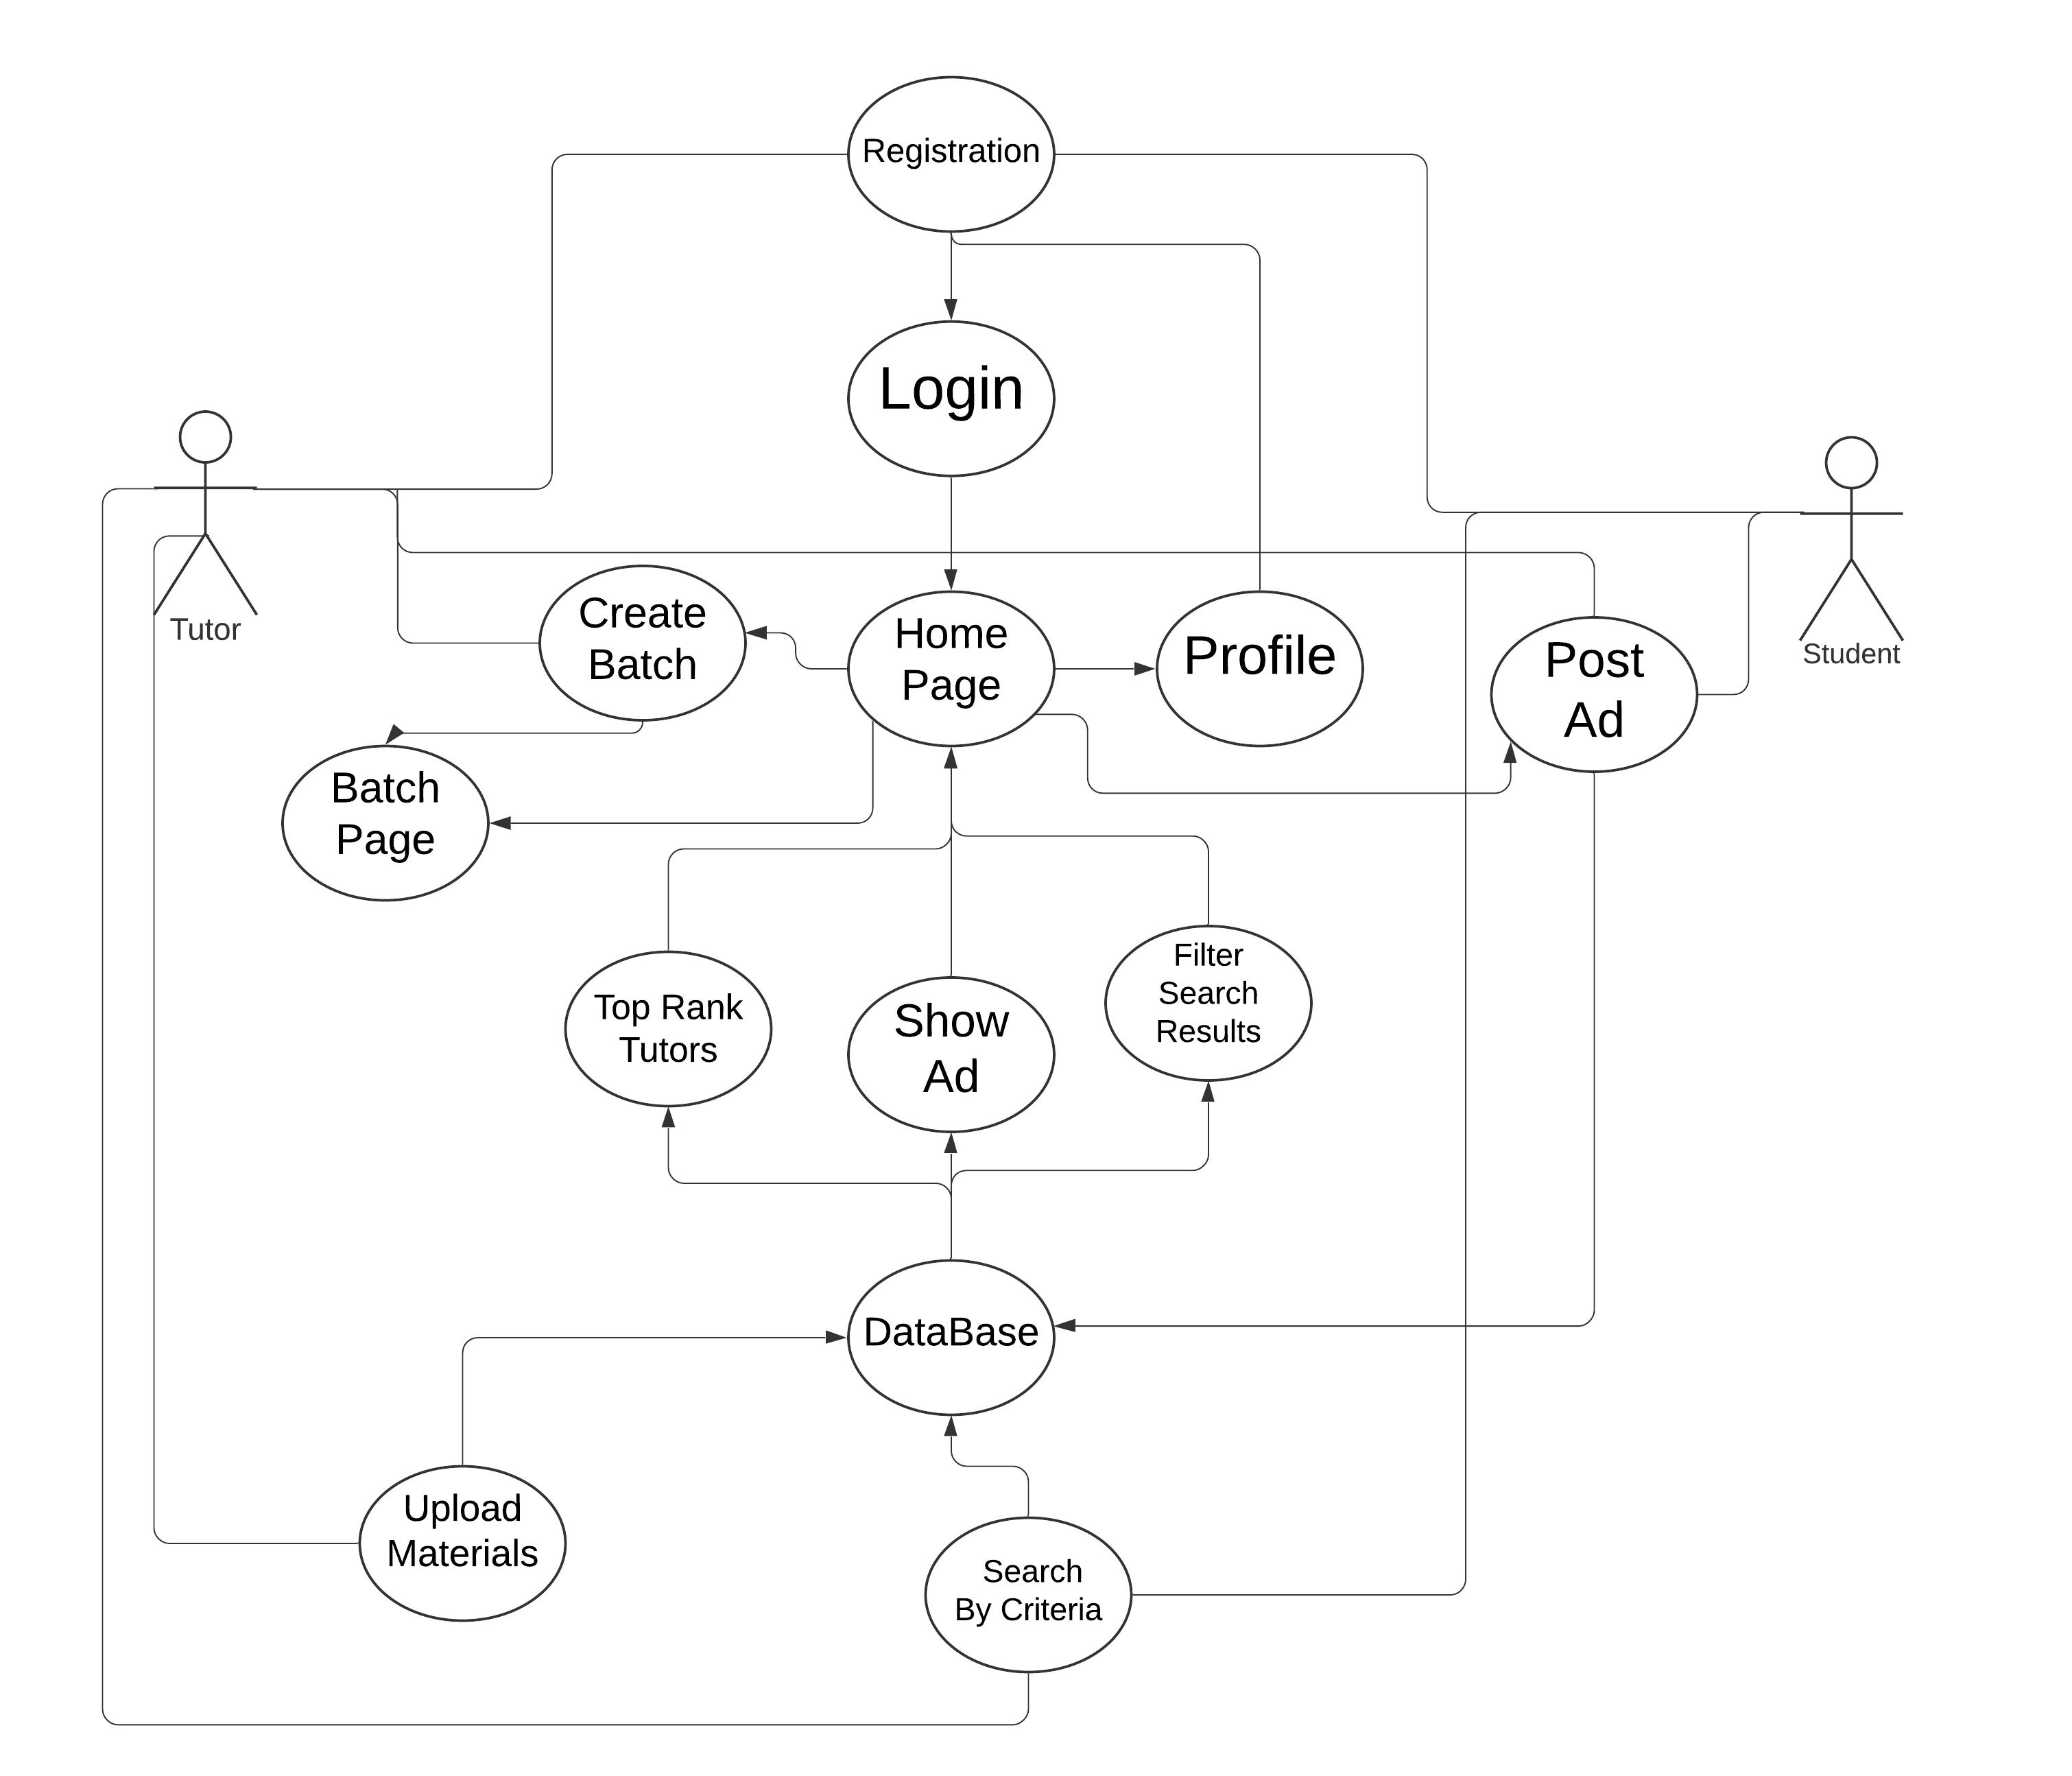
\includegraphics[width=15cm]{images/user_class_diagram.png}
    \caption{User Class and Characteristics}
    \label{fig:User class and Characteristics}
\end{figure}
\section{User Needs}
This system will help the tutor provide the teaching service and the student or their respective supervisor. They are the primary user of this app. They can log in to this app and find their accurate tuition or tutor. This app will be a place to connect the perfect job or to find an ideal tutor. 

Another help of this system will be note sharing. This app will be a spot to collect or transfer necessary documents to the students. The tutor can easily reach his notes to his student. 

These kinds of features will meet what a user needs to connect with a tutor easily. 


\section{Operating Environment}
To support this client-server environment the Web-Application will be developed with the utilization of web server, database server, and frameworks. Server machine, desktop computer, and mobile device (smartphone) are the hardware to be used in the application. Details requirements for the development and deployment of the applications are described below.

%% Software Requirements for Client Start %%
Software Requirements For Client:-
\begin{center}
\setlength{\tabcolsep}{0.8cm}
\renewcommand{\arraystretch}{1.2}
   % \begin{table}[ht]
        \centering
        \begin{longtable}{|m{90pt}|p{9cm}|}
            \hline
                \textbf{Software Name} &\textbf{ Description}\\
            \hline
                \textbf{Sqlite3} &
                    \begin{itemize}
                        \item  Server database
                        \item Provide platform to host client
                        \item application server and
                        \item database for Web application
                    \end{itemize}\\
            \hline
        \end{longtable}
   % \end{table}
\end{center}
%% Software Requirements for Client end %%
%% Hardware Requirements for Client Start %%
\textbf{Hardware Requirements For Client:-}
\begin{center}
\setlength{\tabcolsep}{0.8cm}
\renewcommand{\arraystretch}{1.2}
   % \begin{table}[ht]
        \centering
        \begin{longtable}{|m{90pt}|p{9cm}|}
            \hline
                \textbf{Hardware Name} &\textbf{ Description}\\
            \hline
                \textbf{Client Machine} &
                    \begin{itemize}
                        \item Desktop computer with browser software and Internet connection.
                        \item Smart Phone with browser software and Internet connection.
                        \item Used by system admin to access client as Web-based application in desktop  environment.
                    \end{itemize} \\
            \hline
        \end{longtable}
   % \end{table}
\end{center}
%% Hardware Requirements for Client end %%




%% Software Requirements for Server Start %%
\textbf{Software Requirements For Server:-}
\begin{center}
\setlength{\tabcolsep}{0.8cm}
\renewcommand{\arraystretch}{1.2}
   % \begin{table}[ht]
        \centering
        \begin{longtable}{|m{90pt}|p{9cm}|}
            \hline
                \textbf{Software Name Name} & \textbf{Description}\\
            \hline
                \textbf{Any IDE} &
                    Preferably Visual Studio Code, it enables users to install third-party packages and themes to customize the features and looks of the editor.\\
            \hline
               \textbf{ Python , Django} &
                    \begin{itemize}
                        \item  Python is an Object-Oriented-Programming Language.
                        \item  Django is a Web-Application Frame Work.
                        \item   To run this software locally, Python and Django must be installed on that computer.
                    \end{itemize} \\
            \hline
                \textbf{Sqlite3} &
                    \begin{itemize}
                        \item  Server database
                        \item Provide platform to host client
                        \item application server and
                        \item database for Web application
                    \end{itemize}\\
            \hline
        \end{longtable}
   % \end{table}
\end{center}
%% Software Requirements for Client end %%


%% Hardware Requirements for Server Start %%
\textbf{Hardware Requirements For Server:-}
\begin{center}
\setlength{\tabcolsep}{0.8cm}
\renewcommand{\arraystretch}{1.2}
   % \begin{table}[ht]
        \centering
        \begin{longtable}{|m{90pt}|p{9cm}|}
            \hline
                \textbf{Hardware Name} & \textbf{Description}\\
            \hline
                \textbf{Development PC} &
                    \begin{itemize}
                        \item  Computer installed with all require software and libraries described in Software requirement section.
                        \item  The software being developed will be running under Windows 10 Operating system.
                    \end{itemize} \\
            \hline
                \textbf{Mobile Device} &
                    \begin{itemize}
                        \item  The mobile platform with internet connection where mobile server applications are to be installed
                        \item  Used by student, tutor and parents to access services provided by client in mobile environment.
                    \end{itemize} \\
            \hline
        \end{longtable}
   % \end{table}
\end{center}
%% Hardware Requirements for server end %%

\section{Constraints}
\textbf{Hardware Constraints:} Some of the users of this system will not have high-end computers with which to access this module. Therefore, we must take into account processing and internet speed limitations when designing the system. 

\textbf{Software Constraints:} The \textbf{“Tutor-Hub”} system shall be compatible with the most used multi platform web browsers, Mozilla Firefox, Google Chrome , Safari, Opera Mini, Microsoft Edge  and many more. Since this is a web app system, thus it doesn't have any operating system constraints. For Development purpose There may be purchased components, components reused from another application, or components being developed for subsystems outside of the scope of this SRS, but in order to interact this software application must have :-

\begin{enumerate}
\item Any operating system but Windows and Linux operating systems is preferred .
\item The software should be connected to a web server which runs 24x7.
\item The user accessing/developing the system from any computer must have an internet connection with all browsing capabilities.
\end{enumerate}

\textbf{Communication Constraints:} Below is a list of communication devices or protocols with which the product must interact.For example:-

\begin{enumerate}
\item System must be able to communicate with the printer in order to print documents.
\item System must communicate through TCP/IP port.
\item System is limited to HTTP/HTTPS Protocols only.
\end{enumerate}

.\textbf{Interface with System Constraints:} This system will have to utilise other functions within the existing system, and thus we will be constrained by any existing limits of this system. Possibility of Lack of reference on existing systems.GUI is available only in English.

\textbf{Design and Implementation Constraints:} Some of the design and implementation constraints identified are listed below: 

\begin{enumerate}
\item  Students are allowed to register for more than one course.
\item  Students don't have the authority to edit or access data in the system.
\item  This system supports distributed databases such as Sqlite3.
\item This system may only allow booking but does not include online payment methods. 
\end{enumerate}


\section{Assumptions}
It is assumed that the system follows the Asian localized standard for the course organization.The requirements shall change if the \textbf{“Tutor-Hub”} system is intended to be universal, and any user can belong to a s intended to be universal, and any user can belong to a different organization with their particular database system.

It is assumed that students/tutors data will be made available for the project in some phase of its completion. Until that, test data will be used for providing the demo for the presentations.It is assumed that the students and parents are familiar with applications that find themselves easier .

\begin{enumerate}
\item The users have sufficient knowledge of computers.
\item The remote computer should have Internet connection and Internet server capabilities.
\item The users know the English language, as the user interface will be provided in English
\item This system will not be violating any internet ethnic or cultural rules and won’t be blocked by any Telecom companies.
\end{enumerate}


\newpage




\chapter{Requirements}
\label{Requirements}

%\section{User Interfaces}

\section{Functional Requirements}

%%Functional Requirements-1 Start %%
\textbf{1.Authentication Based Login System :- Registration}
\begin{center}
\setlength{\tabcolsep}{0.8cm}
\renewcommand{\arraystretch}{1.2}
   % \begin{table}[ht]
        \centering
        \begin{longtable}{|m{70pt}|p{9cm}|}
            \hline
                \textbf{Card} &
                    As a user, I want to register with my Google account so that system can authenticate me.\\
            \hline
                \textbf{Conversation} &
                    As a user, I want to register myself with my Google account, then it will save my time as I don't have to enter all of my data by myself.\\
            \hline
                \textbf{Confirmation} & 
                    \textbf{Success:}
                            \begin{itemize}
                            \item  Registered successfully
                            \item  Valid user will be redirected to the login page
                            \end{itemize}
                    \textbf{Failure:}       
                            \begin{itemize}
                            \item  No database connected
                            \item  Service not available
                            \item  Page can't be redirected, Please reload again
                            \end{itemize}\\
            \hline
                \textbf{Conditions of Satisfaction} &  
                        User must be 13years old or above to register account. \\
            \hline
        \caption{Authentication Based Register Account}
        \label{tab:my_label}
        \end{longtable}
   % \end{table}
\end{center}
%%Functional Requirements-1 End %%

%%Functional Requirements-2 Start %%
\textbf{2.Authentication Based Login System :- Login}
\begin{center}
\setlength{\tabcolsep}{0.8cm}
\renewcommand{\arraystretch}{1.2}
   % \begin{table}[ht]
        \centering
        \begin{longtable}{|m{70pt}|p{9cm}|}
            \hline
                \textbf{Card} &
                As a user, I want to login with my Google account so that system can authenticate me.\\
            \hline
                \textbf{Conversation} &
                    As a user, when I go to the login page and login with my Google account, then it will save my time as I don't need to register beforehand to login. \\
            \hline
                \textbf{Confirmation} & 
                    \textbf{Success:} 	
                        \begin{itemize}
                        \item Valid user will be redirected to the homepage
                        \end{itemize}

    	            \textbf{Failure:}
                        \begin{itemize}
                        \item No database connected
                        \item Service not available
                        \item Page can't be redirected, Please reload the page again
                        \end{itemize} \\
            \hline
                \textbf{Conditions of Satisfaction} &  
                        User must have a registered account. \\
            \hline
        \caption{Authentication Based Login}
        \label{tab:my_label}
        \end{longtable}
   % \end{table}
\end{center}
%%Functional Requirements-2 End %%

%% Functional Requirements-3 Start %%
\textbf{3.Authentication Based Login System :- Reset password}
\begin{center}
\setlength{\tabcolsep}{0.8cm}
\renewcommand{\arraystretch}{1.2}
   % \begin{table}[ht]
        \centering
        \begin{longtable}{|m{70pt}|p{9cm}|}
            \hline
                \textbf{Card} &
                As a user, I want to reset my password so that I can secure my login.\\
            \hline
                \textbf{Conversation} &
                    As a user, I want to reset my password in case I have misplaced my previous password. \\
            \hline
                \textbf{Confirmation} &
                     \textbf{ Success:}
                        \begin{itemize}
                            \item  Redirected to the personal information page
                            \item  Enter New Password
                            \item  Confirm Password
                            \item   Password has been reset successfully
                        \end{itemize}
                    \textbf{Failure:}
                        \begin{itemize}
                            \item  No database connected
                            \item  Service not available
                            \item  Page can't be redirected, Please reload again
                        \end{itemize}  \\
            \hline
                \textbf{Conditions of Satisfaction} &  
                    Passwords must contain at least 5 characters. \\
            \hline
        \caption{Authentication Based Reset Password}
        \label{tab:my_label}
        \end{longtable}
   % \end{table}
\end{center}
%% Functional Requirements-3 end %%

%% Functional Requirements-4 Start %%
1.Authentication Based Login System :- Delete Account
\begin{center}
\setlength{\tabcolsep}{0.8cm}
\renewcommand{\arraystretch}{1.2}
   % \begin{table}[ht]
        \centering
        \begin{longtable}{|m{70pt}|p{9cm}|}
            \hline
                \textbf{Card} &
                    As a user, I want to delete my account as i don't need tuition anymore, so that my tuition history is erased.\\
            \hline
                \textbf{Conversation} &
                    As a user, I want to delete my account so that when I don't need the web application anymore; my data is removed from the system.\\
            \hline
                \textbf{Confirmation} &
                     \textbf{ Success:}
                        \begin{itemize}
                            \item Redirected to the personal information page
                            \item  Delete Account
                            \item  Enter password to Confirm
                            \item  Deleted Account Successfully
                        \end{itemize}  
                    \textbf{Failure:}
                        \begin{itemize}
                            \item  No database connected
                            \item    Service not available
                            \item   Page can't be redirected, Please reload again
                        \end{itemize} \\
            \hline
                \textbf{Conditions of Satisfaction} &  
                    user must be registered and logged in to the account.\\
            \hline
        \caption{Authentication Based Delete Account}
        \label{tab:my_label}
        \end{longtable}
   % \end{table}
\end{center}
%% Functional Requirements-4 end %%

%% Functional Requirements-5 Start %%
\textbf{5.Editable profile for both tutor/student:}
\begin{center}
\setlength{\tabcolsep}{0.8cm}
\renewcommand{\arraystretch}{1.2}
   % \begin{table}[ht]
        \centering
        \begin{longtable}{|m{70pt}|p{9cm}|}
            \hline
                \textbf{Card} &
                As a user I want to view and update my user profile's details whenever I want so that my information are updated with present time.\\
            \hline
                \textbf{Conversation} &
                    As a user, I want to view and update my profile so that I can provide my latest information to the system.\\
            \hline
                \textbf{Confirmation} &
                     \textbf{ Success:}
                        \begin{itemize}
                            \item redirected to the personal information page
                            \item View information
                            \item  Edit information
                            \item Save changes
                            \item  View the new information
                        \end{itemize}
                    \textbf{Failure:}
                        \begin{itemize}
                            \item No database connected
                            \item Something went wrong, Try again
                            \item Failed to load the page
                        \end{itemize}\\
            \hline
                \textbf{Conditions of Satisfaction} &  
                    Users must enter their password for security reasons.\\
            \hline
        \caption{Editable Profile for Student/tutor}
        \label{tab:my_label}
        \end{longtable}
   % \end{table}
\end{center}
%% Functional Requirements-5 end %%

%% Functional Requirements-6 Start %%
\textbf{6.Showing Ads:- Find tutor and Find Tuition on both users end}
\begin{center}
\setlength{\tabcolsep}{0.8cm}
\renewcommand{\arraystretch}{1.2}
   % \begin{table}[ht]
        \centering
        \begin{longtable}{|m{70pt}|p{9cm}|}
            \hline
                \textbf{Card} &
                    As a user, I want to see the job posts/ tutors posts on my home page so that i can book tuition easily.\\
            \hline
                \textbf{Conversation} &
                    As a user, when I go to the home page it will show me current job posts of other users. So that, I have the option to choose according to my preferences.  \\
            \hline
                \textbf{Confirmation} &
                     \textbf{ Success:}
                        \begin{itemize}
                            \item   Registered users will see cards of different job ads.
                            \item View more details after pressing see more. 
                            \item Results will show according to recent job ads. 
                        \end{itemize}
                    \textbf{Failure:}
                        \begin{itemize}
                            \item No database connected
                            \item No ads are available
                            \item Page can't be redirected, Please reload the page again
                        \end{itemize}\\
            \hline
                \textbf{Conditions of Satisfaction} &  
                    Users must register themselves to view these ads. \\
            \hline
        \caption{Showing Ads:- Find tutor and Find Tuition for both users}
        \label{tab:my_label}
        \end{longtable}
   % \end{table}
\end{center}
%% Functional Requirements-6 end %%

%% Functional Requirements-7 Start %%
\textbf{7.Create posts to seek tuition/tutor}
\begin{center}
\setlength{\tabcolsep}{0.8cm}
\renewcommand{\arraystretch}{1.2}
   % \begin{table}[ht]
        \centering
        \begin{longtable}{|m{70pt}|p{9cm}|}
            \hline
                \textbf{Card} &
                As a user, I want to post an ad according to my requirements so that i can get tuition/tutor based on my requirements easily.\\
            \hline
                \textbf{Conversation} &
                    As a user, when I will see the tutors requirement is not fulfilling my demands, I want to post my own ads to seek for perfect tutors.\\
            \hline
                \textbf{Confirmation} &
                     \textbf{ Success:}
                        \begin{itemize}
                            \item Registered users will be able to post job ads.
                            \item Ads will be dependent on users preferences.
                            \item Users can put Title, Days, Salaries, Areas
                        \end{itemize}
                    \textbf{Failure:}
                        \begin{itemize}
                            \item No database connected
                            \item Required data is not fulfilled 
                            \item Page can't be redirected, Please reload the page again
                        \end{itemize}\\
            \hline
                \textbf{Conditions of Satisfaction} &  
                        \begin{itemize}
                            \item Users must register themselves to post these ads. 
                            \item To post an ad, users must put proper title, days, salary and location
                        \end{itemize}\\
            \hline
        \caption{Create posts to seek tuition/tutor}
        \label{tab:my_label}
        \end{longtable}
   % \end{table}
\end{center}
%% Functional Requirements-7 end %%


%% Functional Requirements-8 Start %%
\textbf{8. View  post details}
\begin{center}
\setlength{\tabcolsep}{0.8cm}
\renewcommand{\arraystretch}{1.2}
   % \begin{table}[ht]
        \centering
        \begin{longtable}{|m{70pt}|p{9cm}|}
            \hline
                \textbf{Card} &
                As a user, I want to see the details of an ad/post which is posted on the home page or found in the search results.\\
            \hline
                \textbf{Conversation} &
                    As a user, in all ads/posts I will find an option to view the details of the ad so that I can get perfect tuition/tutor for myself. \\
            \hline
                \textbf{Confirmation} &
                     \textbf{ Success:}
                        \begin{itemize}
                            \item  Users will see an option named ‘see more’.
                            \item User presses see more button and system checks and confirms the user is qualified to view more details.
                            \item Users will see full details of the ad in a page. 
                            \item  
                        \end{itemize}
                    \textbf{Failure:}
                        \begin{itemize}
                            \item User clicks see more button.
                            \item System checks and confirms the user is qualified to view more details.
                            \item System denied to redirect users to full details page.
                            \item User is unable to view more details.
                            \item No database connected.
                            \item No ads are available.
                            \item Page can't be redirected, Please reload the page again.
                        \end{itemize} \\
            \hline
                \textbf{Conditions of Satisfaction} &  
                    Users must register themselves to view posts and more details.\\
            \hline
        \caption{View Posts Details}
        \label{tab:my_label}
        \end{longtable}
   % \end{table}
\end{center}
%% Functional Requirements-8 end %%

%% Functional Requirements-9 Start %%
\textbf{9.Search ads based on area/salary/days/subjects/class}
\begin{center}
\setlength{\tabcolsep}{0.8cm}
\renewcommand{\arraystretch}{1.2}
   % \begin{table}[ht]
        \centering
        \begin{longtable}{|m{70pt}|p{9cm}|}
            \hline
                \textbf{Card} &
                 As a user, I want to search job posts/ tutors posts on my home page\\
            \hline
                \textbf{Conversation} &
                     As a user, when I go to the home page after logging in, it will show me a search bar to search for my desired job/tutor. I need to search for a job/tutor where I can select areas, salary, days, subjects and class. Therefore, I have the opportunity to find a job/tutor according to my preferences. \\
            \hline
                \textbf{Confirmation} &
                     \textbf{ Success:}
                        \begin{itemize}
                            \item Registered users will see a search bar above the home page.
                            \item Users need to select area, salary, days, subjects and class to search for a job/tutor.
                            \item User will press the search button.
                            \item System checks and confirms the user is qualified for searching ads.
                            \item Results will show ads according to the selection of the user.
                        \end{itemize}
                    \textbf{Failure:}
                        \begin{itemize}
                            \item Users will select the criteria to search.
                            \item User presses the search button.
                            \item System checks and confirms the user is qualified for searching ads.
                            \item Users cancel the process/system denies the process.
                            \item User is unable to see the results.
                            \item No database connected.
                            \item No ads are available.
                            \item Page can't be redirected, Please reload the page again. 
                        \end{itemize}\\
            \hline
                \textbf{Conditions of Satisfaction} &  
                    \begin{itemize}
                        \item  Users must register themselves to search for an ad.
                        \item Users must select  area, salary, days, subjects and class to search for an ad.
                    \end{itemize}\\
            \hline
        \caption{Search ads based on requirements}
        \label{tab:my_label}
        \end{longtable}
   % \end{table}
\end{center}
%% Functional Requirements-9 end %%


%% Functional Requirements-10 Start %%
\textbf{10.Review and Complain on Tutor}
\begin{center}
\setlength{\tabcolsep}{1.0cm}
\renewcommand{\arraystretch}{1.5}
   % \begin{table}[ht]
        \centering
        \begin{longtable}{|m{70pt}|p{9cm}|}
            \hline
                Card & 
                    As a student/parent, I want to give a review to a tutor so that based on my tuition experience others can decide. \\
            \hline
                Conversation &
                    As a student, after taking tuition from an individual tutor I want to give my reviews as points/stars and write my tuition experiences as comment, so that others who are willing to take tuition from him in future  can gather idea about tutors past activities\\
            \hline
                Confirmation &
                   \textbf{ Success:}
                        \begin{itemize}
                            \item Students/Parents click on the homepage to see the available list of top ranked tutors.
                            \item  System check and confirm parents/students qualified to see top ranked tutors Details on display
                        \end{itemize}
                   \textbf{ Failure}
                        \begin{itemize}
                            \item    Parents/students  click the comment button.
                            \item System check and confirm parents/students qualified to give reviews for the tutor and then display the form to let parents/students write.
                            \item Parents/students enter the comment then submit to the system.
                            \item Parents/students cancel the process.
                            \item System display users cancel results on screen. 
                            \item No database connected.
                            \item Required data is not fulfilled .
                            \item Page can't be redirected, Please reload the page again.
                        \end{itemize}\\
            \hline
                Conditions of Satisfaction &
                    \begin{itemize}
                        \item  Users must register themselves to give  reviews to a tutor
                        \item To give a review, users must put their words in a Ethical manner.
                    \end{itemize} \\
            \hline
        \caption{Review and Complain on Tutor}
        \label{tab:my_label}
        \end{longtable}
  %  \end{table}
\end{center}
%\clearpage
%% Functional Requirements-10 end %%
%% Functional Requirements-10 Start %%
\textbf{10. Feature Top Rank Tutor( On homepage)}
\begin{center}
\setlength{\tabcolsep}{0.8cm}
\renewcommand{\arraystretch}{1.2}
   % \begin{table}[ht]
        \centering
        \begin{longtable}{|m{70pt}|p{9cm}|}
            \hline
                \textbf{Card} &
                    As a student/parent, I want to show a list of top ranked teachers on the system so that I can take tuition from the best ones.\\
            \hline
                \textbf{Conversation} &
                     From the perspective of a student I want to take tuition from the best teachers around my area. From the perspective of a parent I want to provide the best tuition to my children. I want to see a list of top tutors around my area, so that I can select a suitable tutor among them.\\
            \hline
                \textbf{Confirmation} &
                     \textbf{ Success:}
                        \begin{itemize}
                            \item Students/Parents click on the homepage to see the available list of top ranked tutors.
                            \item System check and confirm parents/students qualified to see top ranked tutors Details on display.
                            \item Display Top Ranked Tutors Details.
                        \end{itemize}
                    \textbf{Failure:}
                        \begin{itemize}
                            \item  Students/Parents click on the homepage to see the available list of top ranked tutors.
                            \item System check and confirm parents/students qualified to see top ranked tutors Details on display
                            \item Parents/students cancel the process.
                            \item System display users cancel results on screen and redirected to Homepage.
                            \item No database connected.
                            \item Page can't be redirected, Please reload the page again.
                        \end{itemize}\\
            \hline
                \textbf{Conditions of Satisfaction} &  
                    Users must register themselves to see Top Ranked Tutor.\\
            \hline
        \caption{Feature Top Ranked Tutor}
        \label{tab:my_label}
        \end{longtable}
   % \end{table}
\end{center}
%% Functional Requirements-11 end %%



%% Functional Requirements-12 Start %%
\textbf{12.Platform for Course Materials}
\begin{center}
\setlength{\tabcolsep}{1.0cm}
\renewcommand{\arraystretch}{1.5}
  %  \begin{table}[ht]
        \centering
        \begin{longtable}{|m{70pt}|p{9cm}|}
            \hline
               \textbf{ Card} &
                    As a student, I want an online class platform on the system so that I can attend tuition, view uploaded materials, attend quizzes, submit assignments to the system.\\
            \hline
                \textbf{Conversation} &
                    From the perspective of a student I want  a platform to attend tuition,view lecture materials uploaded by the tutor, Show quizzes questions and submit answers scripts, and also want to see other class members who are taking tuition in the same batch. \\	
            \hline
                \textbf{Confirmation} &
                    \textbf{Success:}
                        \begin{itemize}
                            \item  Students click on the Batch Page to access Course Materials
                            \item  System check and confirm students qualified to see course materials.
                            \item   Students can see uploaded materials on the system.
                            \item   Students can download documents such as notes and exercises, tutors or upload notes.
                        \end{itemize}
                    \textbf{Failure:}
                        \begin{itemize}
                            \item Students click on the batch page to enter.. 
                            \item  System checks and confirms students are qualified to enter and see the course materials page.
                            \item  System cancels the process.
                            \item  System display user cancel result on screen. 
                            \item  No database connected.
                            \item  Page can't be redirected, Please reload the page again.
                        \end{itemize}\\
            \hline
               \textbf{ Conditions of Satisfaction} &
                    Users must register themselves in an online batch to see course materials. \\
            \hline
        \caption{Platform For Course Materials}
        \label{tab:my_label}
        \end{longtable}
  %  \end{table}
\end{center}
%% Functional Requirements-12 end %%


\section{Non Functional Requirements}

\textbf{Performance Requirements:}
\begin{enumerate}
\item The database shall be able to accommodate a minimum of 3,000 records of students.
\item The software shall support use of multiple users at a time. There are no other specific performance requirements that will affect development.
\end{enumerate}
\textbf{Safety Requirements:}
\begin{enumerate}
\item The database may get crashed at any certain time due to virus or operating system failure. Therefore, it is required to take the database backup and the system will ensure data safety.
\end{enumerate}
\textbf{ Security Requirements:}\newline\newline
Some of the factors that are identified to protect the software from accidental or malicious access, use, modification, destruction, or disclosure are described below:-      
\begin{itemize}
\item Keep specific log or history data sets
\item Assign certain functions to different modules.
\item Restrict communications between some areas of the program
\item Communication needs to be restricted when the application is validating the user or license. For example, using https.
\item Username will be unique, the user can not create an account using the same username.
\item Every user is required to have a strong password. Eg: numbers, characters and capital and small letters. 
\item The web-app should be capable enough to handle any kind of common Cyber attacks, like: SQL injection, RCE, CSRF, XSS, LFI/RFI.
\item Restrict communications between some areas of the program
\item Privacy of information, every user's password will be hashed. So, in case of data breach. Passwords won’t be visible. 

\end{itemize}
\textbf{Software Quality Attributes:}

\begin{enumerate}
\item The Quality of the System is maintained in such a way so that it can be very user friendly to all the users.
\item The software should be portable. So moving from one OS to another OS does not create any problem.
\item  The software quality attributes are assumed as under:
\end{enumerate}
			
\begin{itemize}
\item Accurate and hence reliable
\item Secured
\item Fast speed
\item Compatibity
\end{itemize}


\begin{appendices}
\chapter{Glossary}

%% Glossary Table %%

\begin{center}
\setlength{\tabcolsep}{1.0cm}
\renewcommand{\arraystretch}{1.5}
    \begin{table}[ht]
        \centering
        \begin{tabular}{|m{60pt}|p{9cm}|}
            \hline
                \textbf{Term} &  \textbf{Definitions} \\
            \hline
                Active Article  &  The document that is tracked by the system; it is a narrative that is planned to be posted to the public website.\\
            \hline
                Author & Person submitting an article to be reviewed. In case of multiple authors, this term refers to the principal author, with whom all communication is made.\\
            \hline
             	Database &  Collection of all the information monitored by this system.\\
            \hline
            	 Editor &  Person who receives articles, sends articles for review, and makes final judgments for publications.\\
            \hline
             	Field &  A cell within a form. \\
            \hline
            	Member &  A member of the Historical Society listed in the HS database. \\
            \hline
           	 	Reader &  Anyone visiting the site to read articles.\\
            \hline
            	Review & A written recommendation about the appropriateness of an article for publication; may include suggestions for improvement. \\
            \hline
            	Reviewer &  A person that examines an article and has the ability to recommend approval of the article for publication or to request that changes be made in the article. \\
            \hline
            	Software Requirements Specification &  A document that completely describes all of the functions of a proposed system and the constraints under which it must operate. For example, this document. \\
            \hline
            	System Admin & Developer team associated with the system \\
                \hline
            User &  Reviewer or Author. \\
            \hline
        \end{tabular}
        \caption{Glossary Table}
        \label{tab:my_label}
    \end{table}
\end{center}




%\chapter{Analysis Models}
%\chapter{To Be Determined List}




%% Functional Requirements-2 Start %%
%Functional Requirements-2
%\begin{center}
%\setlength{\tabcolsep}{1.0cm}
%\renewcommand{\arraystretch}{1.5}
 %   \begin{table}[ht]
 %       \centering
%        \begin{tabular}{|m{70pt}|p{9cm}|}
%            \hline
%                Card &  Card Text \\
%            \hline
%                Conversation &  Conversation Text\\
%            \hline
%                Confirmation & Confirmation Text  \\
%            \hline
%                Conditions of Satisfaction &  Condition Text \\
%            \hline
 %       \end{tabular}
%        \caption{Authentication Based Logout}
%        \label{tab:my_label}
 %   \end{table}
%\end{center}
%% Functional Requirements-2 end %%





%% Functional Requirements-? Start %%
%\begin{center}
%\setlength{\tabcolsep}{0.8cm}
%\renewcommand{\arraystretch}{1.2}
   % \begin{table}[ht]
 %       \centering
 %       \begin{longtable}{|m{70pt}|p{9cm}|}
 %           \hline
 %               \textbf{Card} &
 %               \\
 %           \hline
 %               \textbf{Conversation} &
 %                    \\
%            \hline
%                \textbf{Confirmation} &
%                     \textbf{ Success:}
%                        
%                    \textbf{Failure:}
%                    \\
%            \hline
%                \textbf{Conditions of Satisfaction} &  
%                    \\
%            \hline
%        \caption{Authentication Based ?}
%        \label{tab:my_label}
%        \end{longtable}
   % \end{table}
%\end{center}
%% Functional Requirements-? end %%



\end{appendices}


